\chapter{Program Counter Incrementer and Mux}

As mentioned in the last lab, the program counter is a register that is one word in length.  It holds the address in memory of the next instruction to be fetched and executed.  There are several ways that the program counter is updated:  
\begin{enumerate}
	\item If the program does not branch (via an if statement, while loop, etc), then the program counter should advance to the next address (add 4 bytes) each clock cycle.
	\item If the conditions of a conditional branch are met, then the program counter should be updated with the branch destination address.
	\item If an unconditional branch or jump occurs, then the program counter should be updated with the branch destination address.
	\item If an interrupt or error occurs, then the program counter should be updated with the interrupt or error handler address.
\end{enumerate}
The instructions will be fetched in sequential order the majority of the time.

\section{Incrementer}

We will build a program counter incrementer by making a simple adder.  Later in our computer we will need another adder, so we will re-use this code.  When used as the program counter, we will pass it a 4 because each instruction is 32-bits long (even though it is a 64-bit computer) and we want to increment to the next instruction in memory.  Most machines are byte addressable, because one ASCII character (a char in c/c++) is a byte.  For a machine with 32-bit instructions like we are using, that would mean that each instruction would be 4 bytes later in memory ($32/8=4$ bytes).  Therefore, we will be adding 4 to the program counter each time we want to increment the program counter.

An adder is very simple in Verilog.  There are two inputs (the two numbers to be added) and one output (the result).   All the ports are size word because they hold integers.  

In this lab you will make your own adder and a testbench for the adder.  Your adder module should be called 'adder' and should have inputs of \verb1a_in1 and \verb1b_in1.  The output should be \verb1add_out1.  HINT: this should be very easy.  Verilog is a Hardware Description Language, so use Verilog to describe what you want to do.  Don't make it complicated.  The adder code should be stored in ARM-Lab/code/0\_common/adder.v.  You will need to create this file.

\section{Input Selection via Mux}

We will also need to be able to choose between normal advancing (sequential stepping) and branching (loops, if statements, etc.).  We will use a multiplexor (mux) to do this.  A mux is a simple device that connects one of the inputs to the outputs based on how the selector bit is set.  If the selector is 0 then input 0 is connected to the output, and if the selector is 1 then input 1 is connected to the output.  One interesting addition in this block of code is the addition of a size parameter.  Parameters are passed before the normal ports and are used to configure the code to meet a requirement at the time of construction.  Note parameters are constants and cannot be changed later in the module.  The $=8$ defines the default value if nothing is specified.  In this case we are using parameters to set the number of wires that compose the inputs and output.  In our problem we will need some muxes to switch entire words (64 bits), but later we will also need to switch register addresses (5 bits).  Rather than write two muxes, we will make one and then use the parameter to change the size when they are declared.  The mux starter code is located in ARM-Lab/code/0\_common/mux.v.

\Verilog{Verilog code to make a mux.}{code:mux}{../code/0_common/mux.v}

Create a testbench for the mux.  Note that if the parameter is not set by the testbench, the mux module will set the inputs and outputs to be the default of 8.  We are going to change this to test it as a 64 bit mux.  In your testbench, instead of creating your mux module using \verb1mux UUT(...1, define the parameter as 64 by changing it to be \verb1mux#(64) UUT(...1  You can also do the dot notation as was done for the ports, but there are usually so few paramters you don't need to.  Now come up with good values to test your mux so you are confident it works.

\section{Expected Results Table}
\begin{figure}
	\caption{Expected Results Table}\label{fig:ert_adder_test}
	\begin{center}
		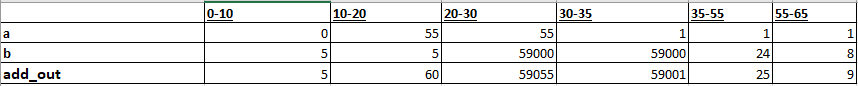
\includegraphics[width=4.75in]{../images/ert_adder_test.png}
	\end{center}
\end{figure} 
In order to verify that our modules work properly, we will create an Expected Results Table and compare our expected results with our simulation results.  The Expected Results Table is not only critical for your own verification of your module, but it is also something that I will use heavily in grading the lab reports.  In your lab reports, I need to be able to easily compare your expected results with your actual results.  Of course, I will examine your test bench code as well so that I can check that your expected results are correct as well.  The Expected Results Table should be done in Excel.  It should have simulation time values across the top and signal names along the left-hand side.  The order of the signal names in your table must match the order of the signal names in your simulation results.  Then you should fill in each block of the table with the expected value for that particular signal at that particular time.  Please use decimal numbers for all values in the expected results and the simulation results. See Figure \ref{fig:ert_adder_test} for an example Expected Results Table.

\section{Your Assignment}

You are to:
\begin{enumerate}
\item Write an adder.	
\item Write a testbench for the adder.
\item Create an Expected Results Table for the adder.
\item Update the mux starter code to operate as a mux.
\item Write a testbench for the mux.
\item Create an Expected Results Table for the mux.
\item Run a simulation and generate a timing diagram for each testbench.
\item Compare your Simulation Results with your Expected Results Table and resolve discrepancies.
\item Write up a lab report in \LaTeX\ following the lab format in \verb1LabN.tex1 and generate a pdf file.
\item Upload the pdf and all the Verilog files to Canvas.
\end{enumerate} 